%!TEX TS-program = xelatex
%!TEX encoding = UTF-8 Unicode
\documentclass[russian,hyperref={unicode}]{beamer}
% Other packages (for math and grahics)
\usepackage{amsmath, amssymb, graphicx, csquotes}
\graphicspath{{../articles/4-rlnc-conference/presentation/images/}}
% Exclude backup slides from numbering
\usepackage{appendixnumberbeamer}
% Theme selection
\usetheme[sectionpage=none, numbering=fraction]{metropolis}
% Locale packages
\usepackage{polyglossia}
\setmainlanguage{russian}
\setkeys{russian}{babelshorthands=true}
\usepackage[backend=biber,
            sorting=nyt,
            bibstyle=gost-authoryear,
            language=auto,
            babel=other,
            doi=false,
            eprint=false,
            isbn=false,
            dashed=false,
            maxbibnames=4,
            ]{biblatex}
\bibliography{../text/bibliography.bib}

\title{Алгоритмы определения пространственной ориентации подвижных объектов в задачах радионавигации}
\institute
{
  Воронежский Государственный Университет \\
  Факультет Компьютерных Наук \\
  Кафедра Цифровых Технологий
}
\author
{
  Выполнил: студент 2 курса маг. Морозов Е.~Ю. \\
  Руководитель: к.~ф.-м.~н.~Минин Л.~А.
}
\date{6 июня 2019 г.}

\begin{document}
  \frame{\titlepage}

  \section{Введение}
  \begin{frame}{Введение}
    В настоящее время большое распространение получили глобальные навигационные спутниковые системы.

    Основная задача таких систем "--- определение координат подвижных объектов.

    Угловая ориентация определяется другими системами (например, VOZ/DME или РСБН) или с помощью вспомогательных навигационных приборов.

    Создание единой системы, позволяющей с требуемой точностью одновременно определять координаты и угловую ориентацию подвижных объектов, является актуальной задачей.~\nocite{WMMU:2019:IIS, WMMU:2019:RLNC, WMM:2018}
  \end{frame}

  \section{Постановка задачи}
  \begin{frame}{Постановка задачи}
    Профессор А.~Д.~Виноградов из Военно-воздушной академии им.~Н.~Е.~Жуковского и Ю.~А.~Гагарина предложил вариант такой системы, основанной на измерении углов с помощью фазированных антенных решеток.

    Источниками сигналов являются радиоориентиры, размещенные в точках с известными координатами.

    Подвижный объект оснащен бортовой пеленгаторной антенной (БПА), способной определять азимут и угол места каждого радиоориентира.
  \end{frame}

  \begin{frame}{Постановка задачи}
    Измерения проводятся в системе координат, связанной с подвижным объектом.

    Всего необходимо определить шесть параметров "--- три координаты фазового центра БПА и три угла Эйлера, определяющих угловую ориентацию подвижного объекта.

    Минимальное число РО равно трем, так как БПА подвижного объекта измеряет два параметра для каждого из радиоориентиров "--- азимут и угол места.
  \end{frame}

  \begin{frame}{Постановка задачи}
    \begin{columns}[c]
      \begin{column}{.5\textwidth}
        %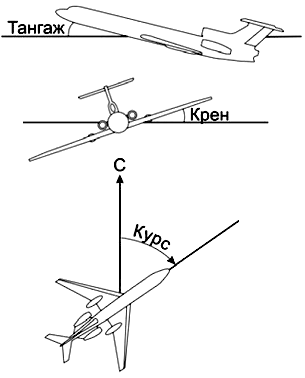
\includegraphics[height=.9\textheight]{yaw_pitch_roll}
      \end{column}
      \begin{column}{.5\textwidth}
        \begin{center}
          %\includegraphics[height=.9\textheight]{coordinates}
        \end{center}
      \end{column}
    \end{columns}
  \end{frame}

  \begin{frame}{Схема решения}
    Можно выделить три этапа решения задачи:
    \begin{enumerate}
        \item Нахождение совокупности расстояний от подвижного объекта до радиоориентиров;
        \item Определение координат подвижного объекта;
        \item Нахождение матрицы вращения и связанных с нею углов Эйлера, определяющих угловую ориентацию подвижного объекта.
    \end{enumerate}
    Задачи второго и третьего этапов являются стандартными для радионавигации подвижных объектов.
  \end{frame}

  \begin{frame}{Схема решения. Первый этап}
    В задаче есть две системы координат:
    \begin{itemize}
      \item \textit{Базовая} или \textit{земная} "--- в ней известны координаты РО и в ней требуется определить координаты объекта;
      \item \textit{Связанная} с подвижным объектом "--- может быть повернута относительно базовой, в ней проводятся измерения направлений на РО.
    \end{itemize}

    По измеренным направлениям можно определить косинусы углов между ними.

    Фактически, решается такая задача: даны длины ребер основания и плоские углы при вершине треугольной пирамиды; найти длины боковых ребер.
  \end{frame}

  \begin{frame}{Схема решения. Первый этап}
    \begin{figure}
      \begin{center}
        \includegraphics[width=.8\textheight]{tetrahedron}

        \caption{Схема размещения в пространстве трех радиоориентиров $M_1$, $M_2$ и $M_3$ и подвижного объекта $M_0$}
        \label{fig:tetrahedron}
      \end{center}
    \end{figure}
  \end{frame}

  \begin{frame}{Схема решения. Первый этап}
    Система уравнений для нахождения расстояний $\ell_1$, $\ell_2$ и $\ell_3$:
    \begin{equation} \label{eq:system}
      \begin{cases}
        \ell_1^2 + \ell_2^2 - 2 \ell_1 \ell_2 \cos\alpha_{12} = d_{12}^2 \\
        \ell_1^2 + \ell_3^2 - 2 \ell_1 \ell_3 \cos\alpha_{13} = d_{13}^2 \\
        \ell_2^2 + \ell_3^2 - 2 \ell_2 \ell_3 \cos\alpha_{23} = d_{23}^2
      \end{cases}
    \end{equation}
    Нелинейная, однородная система второго порядка.
  \end{frame}

  \section{Особенности решения}
  \begin{frame}{Особенности решения. Первый этап}
    Проведенные расчеты, произведенные с помощью Wolfram Mathematica, показали, что система~\eqref{eq:system} имеет от одного до четырех решений. Отсюда возникают три проблемы:
    \begin{enumerate}
      \item Как определить количество решений? \label{q:1}
      \item Как выбрать правильное решение? \label{q:2}
      \item Как оценить погрешность нахождения решения при заданных погрешностях входных данных? \label{q:3}
    \end{enumerate}

  \end{frame}

  \begin{frame}{Особенности решения. Первый этап}
    Систему~\eqref{eq:system} можно свести к уравнению четвертой степени относительно одной переменной. При этом, коэффициент при старшей степени может принимать очень малые значения и даже обращаться в ноль.

    \begin{equation*}
      \begin{array}{l}
      (1-4 \cos^2 \alpha_{23}) b^4 + 4 \cos \alpha_{23} (\cos \alpha_{23} + 2 \cos \alpha_{12} \cos \alpha_{23} ) b^3 - \\
      - 2 (1 + 8 \cos \alpha_{12} \cos \alpha_{13} \cos \alpha_{23}) b^2 +
      \\+ 4 \cos \alpha_{13} (\cos \alpha_{23} + 2 \cos \alpha_{12} \cos \alpha_{13}) b + 1-4 \cos^2 \alpha_{13} =0
      \end{array}
    \end{equation*}

    Предложить устойчивый метод решения такого уравнения не удалось.
  \end{frame}

  \begin{frame}{Особенности решения. Первый этап}
    Минимизирующий функционал ошибок в случае $m$ РО ($m \ge 4$):
    \begin{equation*}
      \Phi\left(\ell_1, \cdots, \ell_m \right) = \frac{1}{2}\sum_{1 \leq j < i \leq m} \left(\ell_i^2 + \ell_j^2 - 2 \ell_i \ell_j \cos\alpha_{ij} - d_{ij}^2\right)^2
    \end{equation*}
    Приравняем к нулю частные производные по $\ell_1, \cdots, \ell_m$:
    \begin{equation*}
      \frac{\partial\Phi}{\partial\ell_k} = \sum_{j \ne k} \left(\ell_k^2 + \ell_j^2 - 2 \ell_k \ell_j \cos\alpha_{kj} - d_{kj}^2\right)\left(2 \ell_k - 2 \ell_j \cos\alpha_{kj}\right) = 0,
    \end{equation*}
    \begin{equation*}
      k = 1, 2, \cdots, m.
    \end{equation*}
    Таким образом, получена система из четырех однородных кубических уравнений относительно четырех неизвестных.
  \end{frame}

  \begin{frame}{Особенности решения. Первый этап}
    Систему~(\ref{eq:system}) можно решать методом Ньютона. Это обусловлено следующим:
    \begin{itemize}
      \item Имеется хорошее начальное приближение;
      \item Быстрая сходимость к решению (5-10 итераций);
      \item В реализации присутствуют только элементарные арифметические действия "--- обратная матрица выписывается явно.
    \end{itemize}

    По итогам компьютерного моделирования С.~Н.~Ушаковым была установлена структура и условия динамика появления паразитных решений.
  \end{frame}

  \section{Заключение}

  \begin{frame}{Вспомогательные задачи}
    В данной работе также рассматриваются другие варианты локальных навигационных систем, в частности, когда в системе присутствует несколько подвижных объектов, или когда подвижный объект оснащен высотомером.

    Также была рассмотрена вспомогательная задача "--- влияние на результаты измерений БПА подстилающей поверхности. В такой ситуации подвижный объект принимает два сигнала "--- исходный и отраженный.
  \end{frame}

  \begin{frame}{Дальнейшие планы}
    Дальнейшие планы заключаются в следующем:
    \begin{itemize}
      \item Произвести оценку погрешностей работы рассмотренной системы;
      \item Сотрудничество с Институтом проблем управления имени В.~А.~Трапезникова;
      \item Подача заявки на патент совместно с А.~Д.~Виноградовым.
      \item Исследование других перспективных конфигураций локальных навигационных систем.
    \end{itemize}
  \end{frame}

  \begin{frame}{Выводы}
    \begin{itemize}
      \item С помощью компьютерного моделирования установлена неоднозначность решения задачи о нахождении расстояний от РО до БПА посредством угловых измерений.
      \item Проведен анализ выбора наилучшего способа решения задачи нахождения расстояний и показано, что метод Ньютона решения систем нелинейных уравнений дает устойчивый способ решения.
      \item Рассмотрены различные конфигурации взаимного расположения подвижных объектов и радиоориентиров и связанные с ними вычислительные и математические задачи.
      \item Изучен вопрос о влиянии отраженного от Земли сигнала при малой высоте подвижных объектов.
    \end{itemize}
  \end{frame}

  \begin{frame}[allowframebreaks]{Список публикаций}
    % \bibliographystyle{amsalpha}
    \printbibliography
  \end{frame}

  \frame{\titlepage}

  \appendix
  \begin{frame}{Визуализация решений, полученных на первом этапе}
    \begin{columns}[c]
      \begin{column}{.5\textwidth}
        \begin{itemize}
          \item В основании "--- равносторонний треугольник
          \item Аппарат изначально находился в центре
          \item Фиолетовым цветом выделены зоны с одним решением
          \item Оранжевым "--- зоны с несколькими решениями
        \end{itemize}
      \end{column}
      \begin{column}{.5\textwidth}
        \begin{center}
          \includegraphics[width=\columnwidth]{tetrahedron-regular}
        \end{center}
      \end{column}
    \end{columns}
  \end{frame}

  \begin{frame}{Визуализация решений, полученных на первом этапе}
    \begin{columns}[c]
      \begin{column}{.5\textwidth}
        \begin{itemize}
          \item В основании также равносторонний треугольник
          \item Аппарат изначально находился рядом с одной из вершин
        \end{itemize}
      \end{column}
      \begin{column}{.5\textwidth}
        \begin{center}
          \includegraphics[width=\columnwidth]{tetrahedron-bifurcation}
        \end{center}
      \end{column}
    \end{columns}
  \end{frame}

  \begin{frame}{Визуализация решений, полученных на первом этапе}
    \begin{columns}[c]
      \begin{column}{.5\textwidth}
        \begin{itemize}
          \item В основании также равносторонний треугольник
          \item Аппарат изначально находился за пределами треугольника
          \item При дальнейшем подъеме аппарата паразитные имеют сложную структуру
        \end{itemize}
      \end{column}
      \begin{column}{.5\textwidth}
        \begin{center}
          \includegraphics[height=.9\textheight]{tetrahedron-away}
        \end{center}
      \end{column}
    \end{columns}
  \end{frame}

  \begin{frame}{Геометрическая интерпретация решений}
    Рассмотрим треугольник, образованный двумя РО ($M_i$, $M_j$) и подвижным объектом $M_0$.

    Так как известен угол $\angle M_i M_0 M_j$, точка $M_0$ может лежать на окружности с хордой $M_i$ $M_j$.

    Геометрическое место точек, в которых может находится $M_0$ при заданных $\ell_{i}$, $\ell_{j}$ и $\angle M_i M_0 M_j$ образуется вращением этой окружности вокруг хорды $M_i$ и $M_j$, образуя \textit{закрытый тор}.

    Пересечение трех закрытых торов, полученных для каждой из сторон, является истинным положением воздушного объекта.
  \end{frame}

  \begin{frame}{Геометрическая интерпретация решений}
    \begin{center}
      \begin{figure}
        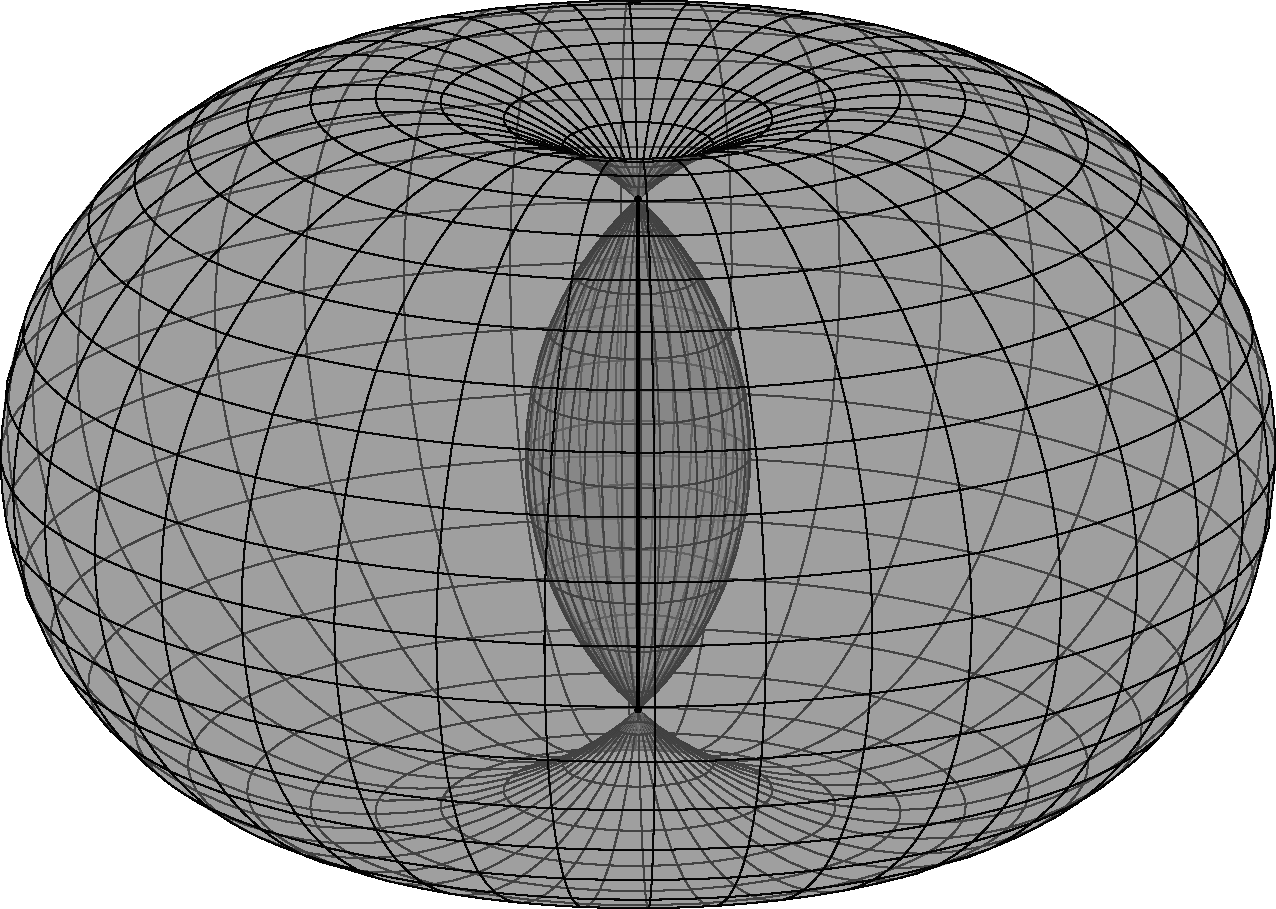
\includegraphics[height=.7\textheight]{torus}
        \caption{Закрытый тор, иллюстрирующий области возможного нахождения подвижного объекта $M_0$ относительно ребра $M_1M_2$.}
      \end{figure}
    \end{center}
  \end{frame}
\end{document}
